\newpage 

\section{Transactions and Concurrency Control}

\noindent
Say the backbone of our stock trading application is a 
distributed database. The system may conduct complicated
stock trades based on server stock prices.
\begin{figure}[h]
    \centering
    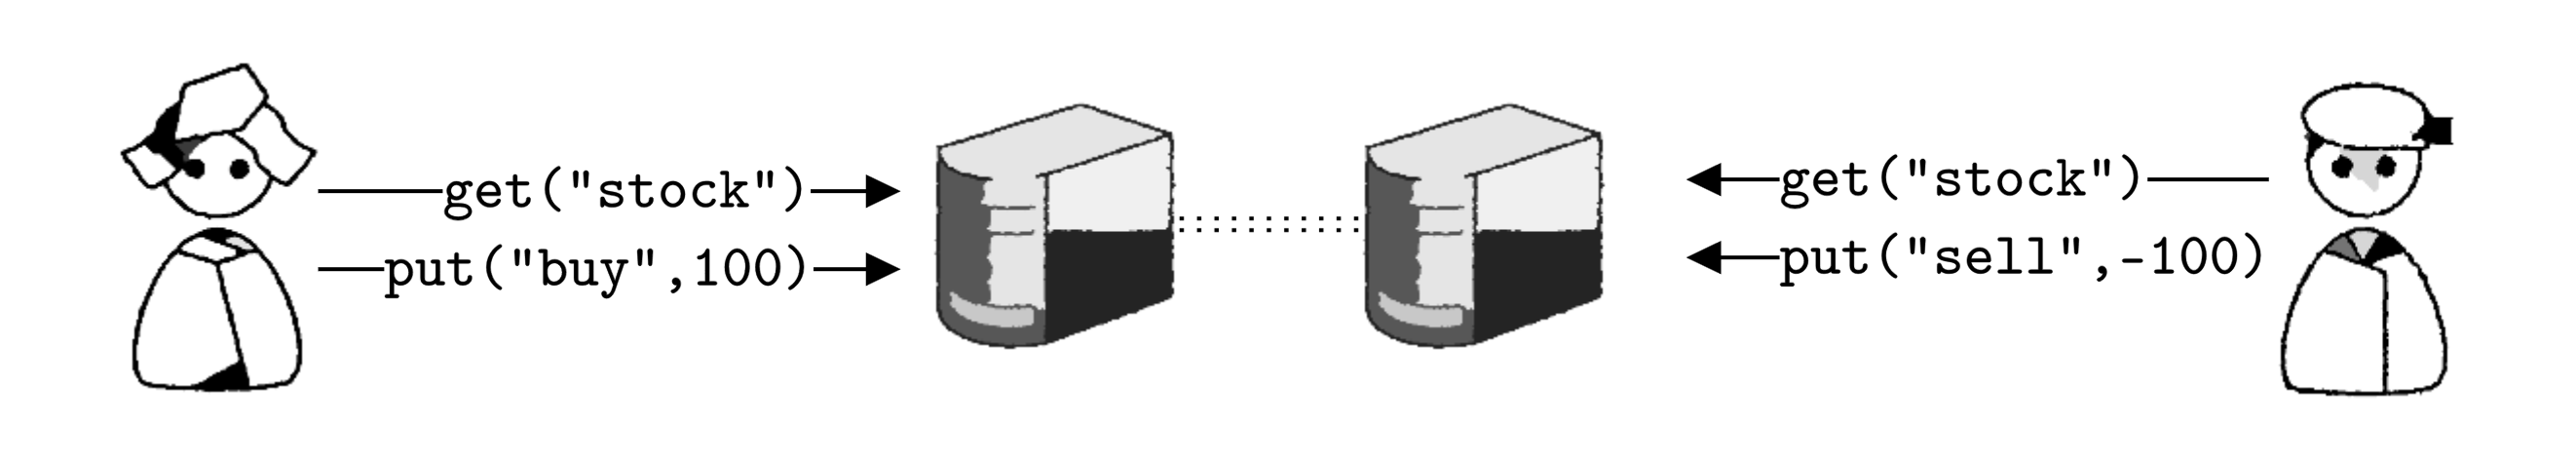
\includegraphics[width=\textwidth]{Sections/trans/stock.png}
    \caption{Two users checking the stock prices and making a trade based on such information.}
    \label{fig:stock_trading}
\end{figure}

\noindent
It is critical that the stock price is consistent through all servers, and 
more important that if any trade fails, the system can recover to a consistent state.

\begin{Def}[Transaction]

    A \textbf{transaction} is a sequence of operations that are treated as a single unit of work.
    A transaction must satisfy the \textbf{ACID} properties:
    \begin{itemize}
        \item \textbf{Atomicity}: A transaction is either fully completed or not executed at all.
        \item \textbf{Consistency}: A transaction must leave the database in a consistent state.
        \item \textbf{Isolation}: Transactions must be isolated from each other.
        \item \textbf{Durability}: Once a transaction is committed, it remains so even in the event of a system failure.
    \end{itemize}
\end{Def}

\vspace{-0.5em}
\begin{figure}[h]
    \centering 
    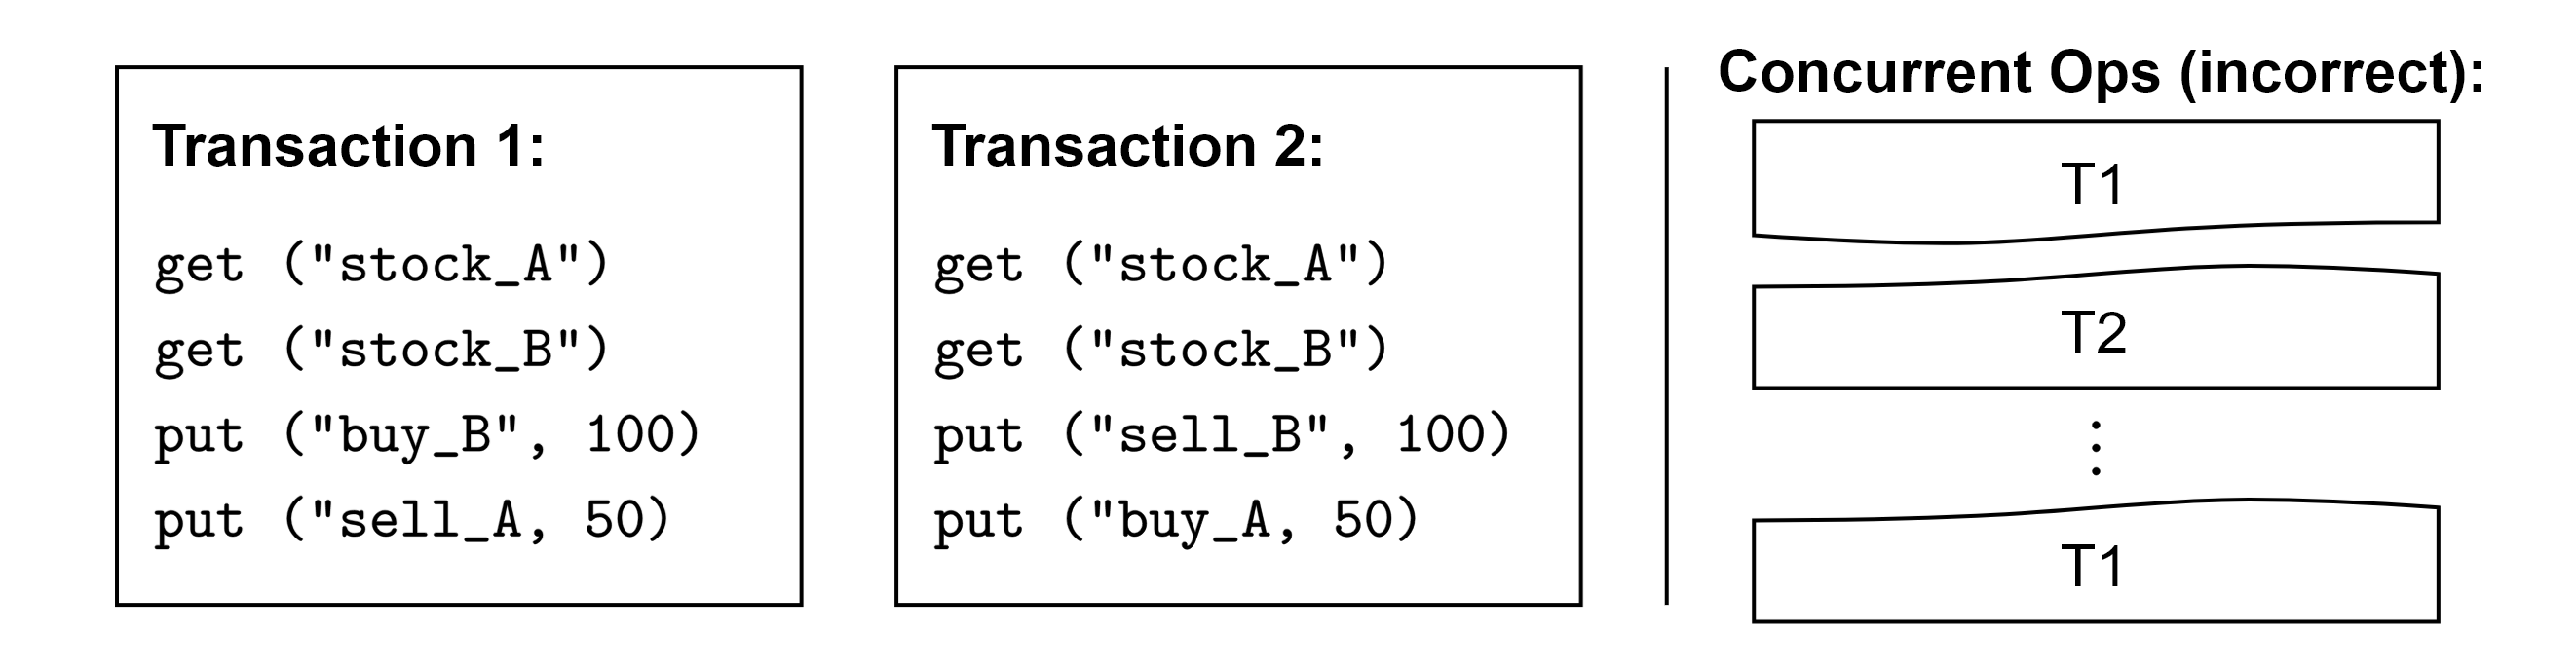
\includegraphics[width=\textwidth]{Sections/trans/stock_2.png}
    \caption{Two transactions which whose operations are interleaved.}
    \label{fig:stock_trading}
\end{figure}

\noindent
Interleaving transactions \textbf{violates the isolation property}. This is problematic in 
Figure (\ref{fig:stock_trading}) as T2's (transaction 2) operations may depend on the server 
state before T1's transaction. Additionally partially completed transactions leave the system in an inconsistent state, violating
\textbf{atomicity}
(e.g., T1's ``buy\_B'' fails, but ``sell\_A'' succeeds).

\newpage

\noindent
There are two standard ways we handle transactions:
\begin{Def}[Optimistic Concurrency Control (OCC)]

    \textbf{Optimistic Concurrency Control (OCC)}: Assumes conflicts are rare, involving three phases:
        \begin{itemize}
            \item \textbf{Read Phase}: Reads transaction requests, creates a temporary copy of the data to preform all operations.
            \item \textbf{Validation Phase}: Once a \textbf{commit point} is reached, the system checks if the 
            transaction is \textbf{serializable}. This means the transaction has some \textbf{serial order}---operations execute sequentially, one after the other in a predictable logical fashion.
            I.e., it guarantees that in the face of interleaving transactions, the result is the same as if operations ran in order on a single thread.\\

            Serializability is a \underline{\textbf{strong consistency model}} as it enforces a strict order of operations.
            This is \textbf{different than linearizability}, which allows for interleaving actions within a \textbf{single} operation in respect to real-time.
            In contrast, serializability concerns the order of \textbf{multiple} operations in respect to serial order.
            \item \textbf{Write Phase}: If the transaction is serializable, the system commits the changes to the database. Otherwise, it \textbf{aborts} the transaction and rolls back to the previous state.
        \end{itemize}

    
\end{Def}
